\documentclass[11pt,a4paper]{article}
\usepackage[
    left=0.73in,
    right=0.73in,
    top=.8in,
    bottom=.50in,
    paperheight=11in,
    paperwidth=8.5in
]{geometry}
\usepackage{array}
\newcolumntype{C}[1]{>{\centering\let\newline\\\arraybackslash\hspace{0pt}}m{#1}}

\usepackage{graphicx}
\usepackage{textcomp}

\begin{document}
% Cover Page
\pagenumbering{gobble}
\begin{center}
\textbf{
    \Large{ECE 543: Introduction to Digital Systems}
    \\~\\
    \large{Instructor: Bessam Zuhair Al Jewad, Ph.D.}
    \\[1.25in]
    \LARGE{Prelab \#1: Introduction to the global specialties PB505}
    \\[0.62in]
    \large{Prepared for Himadri Basu (TA)\\~\\By Christopher Chin}
    \\[1.25in]
    \LARGE{Section 6}
    \\[1.25in]
    \Large{Department of Electrical and Computer Engineering\\
           University of New Hampshire}
    \\[1.25in]
    \Large{\today}
}
\end{center}
\clearpage
\pagenumbering{arabic}

% TOC
\tableofcontents
\pagebreak

% Pages
\section{Introduction}
The objective of this lab is to become familiar with the lab equipment by testing the modules on
the PB-505 Digital Lab. In addition, the lab will involve the construction of a circuit using the
7486 TTL IC\@.
\section{Equipment Required}
\begin{itemize}
    \item Global Specialties Design and Prototyping PB-505
    \item Wire leads
    \item 7486 TTL Integrated Circuit(1)
\end{itemize}
\section{Procedures}
\subsection{PB-505 Design}
\begin{figure}[ht!]
    \centering
    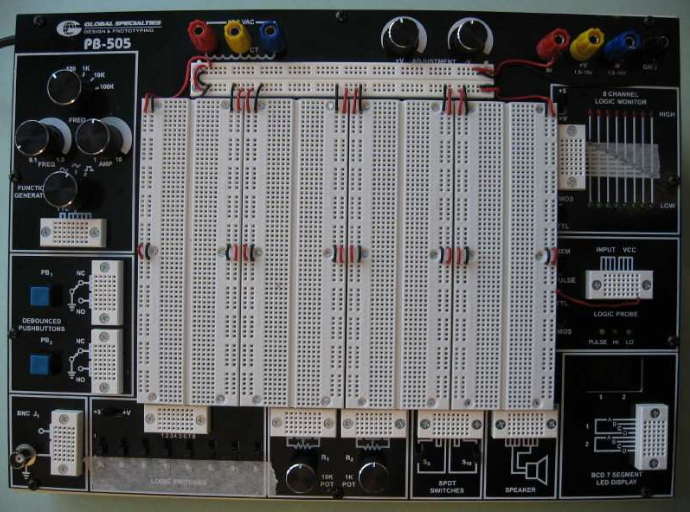
\includegraphics[width=14cm]{breadboard.png}
    \caption{Global Specialties Design and Prototyping PB-505}
\end{figure}
The breadboard has internal connections. There are horizontal connections for each
row of five sockets. There are vertical connections surrounding the horizontal rows.
Those connected to the red wires hold VCC\@. Those connected to the black wires are
ground. The board contains modules such as the Logic Monitor, Logic Probe, Wave
Generator, Pushbuttons, Switches, and Speaker.

% Logic Probe section
\subsection{Circuit Diagrams}
\begin{figure}[ht!]
    \centering
    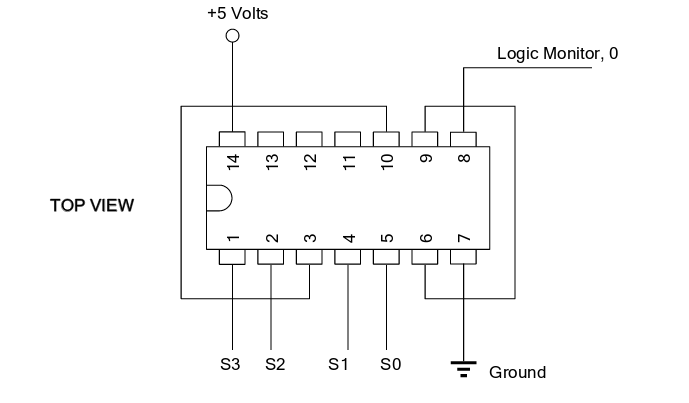
\includegraphics[width=12cm]{IC-wires.png}
\end{figure}

Voltage is attached to pin 14. Ground is attached to pin 7. S0 is connected
to pin 5. S1 to pin 4. S2 to pin 2. S3 to pin 1. Pin 3 on the chip is connected
to pin 10. Pin 6 on the chip is connected to pin 9. Pin 8 is the output.

\subsection{IC Logic Diagrams}
\begin{figure}[ht!]
    \centering
    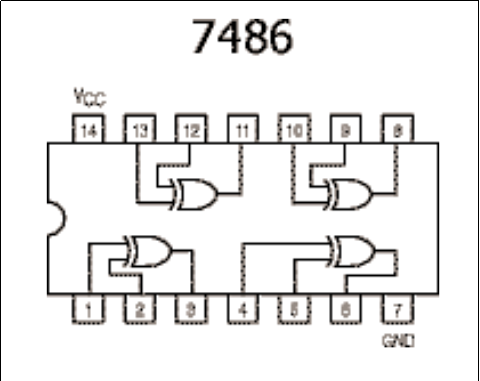
\includegraphics[width=6cm]{logic.png}
    \caption{7486 IC logic diagram}
\end{figure}
The IC takes pin 1 and pin 2 as inputs and outputs the XOR of the two pins to pin 3.
The IC takes pin 4 and pin 5 as inputs and outputs the XOR of the two pins to pin 6.
The IC takes as inputs pin 10 and pin 9 which are connected to pins 3 and 6 and outputs
the XOR of the two pins to pin 8.
Though our circuit does not use them the IC takes pin 12 and pin 13 as inputs and
outputs the XOR of the two pins to pin 11.

\subsection{IC Design}
\begin{figure}[ht!]
    \centering
    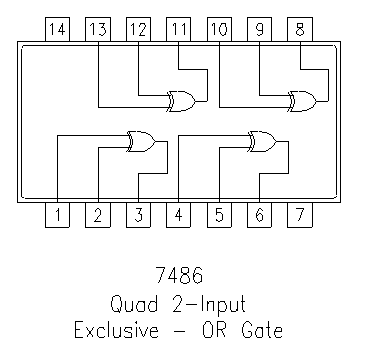
\includegraphics[width=6cm]{pins.png}
    \caption{7486 IC logic diagram}

    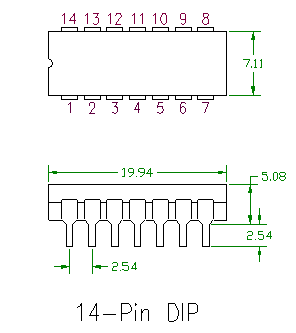
\includegraphics[width=6cm]{dimensions.png}
    \caption{7486 IC dimensions}
\end{figure}
Features:
\begin{itemize}
    \item Four 2-Input Exclusive OR Gates in a 14 Pin DIP package
    \item Outputs directly interface to CMOS, NMOS, and TTL
    \item Large operating voltage range
    \item wide operating conditions
\end{itemize}
\begin{tabular}{l l}
    Supply Voltage & 7V\\
    Input Voltage  & 5.5V\\
    Operating Free Air Temperature  & 0$\textdegree$ C to +70$\textdegree$ C\\
    Storage Temperature Range       & -65$\textdegree$ C to +150$\textdegree$ C\\
\end{tabular}

\subsection{Binary Table}
\begin{tabular}{| C{1.83cm} | C{1.83cm} | C{1.83cm} | C{1.83cm} | C{1.83cm} | C{1.83cm} | C{1.83cm} | }
    \hline
        \multicolumn{4}{|c|}{Inputs}
        & \multicolumn{2}{|c|}{Intermediates}
        & Output \\
    \hline
        S3 & S2 & S1 & S0 & Chip 1, Pin 3 & Chip 1, Pin 6 & Logic Monitor, 0 \\
    \hline
        0  & 0  &  0 &  0 & 0 & 0 & 0\\
    \hline
        0  & 0  &  0 &  1 & 0 & 1 & 1\\
    \hline
        0  & 0  &  1 &  0 & 0 & 1 & 1\\
    \hline
        0  & 0  &  1 &  1 & 0 & 0 & 0\\
    \hline
        0  & 1  &  0 &  0 & 1 & 0 & 1\\
    \hline
        0  & 1  &  0 &  1 & 1 & 1 & 0\\
    \hline
        0  & 1  &  1 &  0 & 1 & 1 & 0\\
    \hline
        0  & 1  &  1 &  1 & 1 & 0 & 1\\
    \hline
        1  & 0  &  0 &  0 & 1 & 0 & 1\\
    \hline
        1  & 0  &  0 &  1 & 1 & 1 & 0\\
    \hline
        1  & 0  &  1 &  0 & 1 & 1 & 0\\
    \hline
        1  & 0  &  1 &  1 & 1 & 0 & 1\\
    \hline
        1  & 1  &  0 &  0 & 0 & 0 & 0\\
    \hline
        1  & 1  &  0 &  1 & 0 & 1 & 1\\
    \hline
        1  & 1  &  1 &  0 & 0 & 1 & 1\\
    \hline
        1  & 1  &  1 &  1 & 0 & 0 & 0\\
    \hline
\end{tabular}

\subsection{Work Done to Complete the Objective}
Test the various modules on the PB-505 Digital Lab. Generate a circuit incorporating the 7486 TTL IC.
\subsection{Predicted Results and Discussion}
\begin{enumerate}
    \item Logic switches should act as on and off switches for leads next to each switch.
    \item Each push button should move GND from NC to NO.
    \item The vertical rows meant for VCC should light the HIGH LED on the lamp monitor.
        The vertical rows meant for GND should light the LOW LEDs.
    \item The logic probe should detect HIGH and LOW Voltages.
    \begin{enumerate}
        \item The probe should read LOW when connected to S7 and S7 is on. The probe should
            not detect any voltage when S7 is off.
        \item The probe should read LOW when connected to NC and the push button is not
            pressed and not have a reading when the push button is pressed.
        \item The PULSE light illuminates whenever voltage changes from 0 to low. When set
            to MEM it should remain illuminated until voltage hits 0.
    \end{enumerate}
\end{enumerate}
\pagebreak
\section{References}
Ronald J. Tocci et al. 2011. Digital Systems: Principles and Applications, 11\textsuperscript{th} Ed.

"7486 - 7486 Quad EXCLUSIVE-OR Gate Datasheet". http://www.futurlec.com/74/IC7486.shtml
\hspace{1cm}Pearson/Prentice Hall.
\end{document}
